% ------ APPENDIX B ------

\chapter{Programmer manual}
% ------ APPENDIX INTRO ------
This appendix explains how the two implementations are designed. In particular, there is a first section about the frameworks and the libraries used, followed by the implementation itself (with code explanations, problems, resolutions, endpoints and messages exchanged in practice) for both the examples. Finally, the last section is devoted to the compilation and dockerization of the solutions.
% ------ END OF APPENDIX INTRO ------

\minitoc

% ------ SECTION B.1 ------
\section{Frameworks, libraries and environment}
For what concerns the second demo and the server of the first demo, it has been used Apache Maven as build automation tool and the only requirement is Java JDK8 installed. Moreover, since Maven is integrated in the project (by using maven-wrapper), there is no need to install it on the machine.
For what concerns the client in the first demo, React is the Javascript framework chosen. Obviously, \texttt{npm} and \texttt{node} must be installed on the machine (see \url{https://www.npmjs.com/get-npm} to get both of them). 
The code of the implementation examples is available on GitHub:

\begin{itemize}
    \item \textbf{\oauth\ with Google/Facebook}\footnote{\url{https://github.com/nopesir/oauth-hw-security}}
    \item \textbf{\oauth\ with custom AuthZ/Resource servers}\footnote{\url{https://github.com/nopesir/oauth-hw-security-custom}}
\end{itemize}

Last but not least, both \texttt{Docker} and \texttt{Docker-Compose} must be installed too in order to dockerize the solutions. For instructions, see (\ref{appa}).
% ------ END OF SECTION B.1 ------

% ------ SECTION B.2 ------
\section{Implementation}
In this section are analyzed design and implementation of the two solutions with messages exchanged and endpoints used. The "Playground" demo provided by OAuth.com in collaboration with Okta \cite{playgr} can be very helpful for the developer in order to understand the flows and the protocol from a practical point of view. 

% ------ SECTION B.2.1 ------
\subsection{\oauth\ with Google/Facebook}
The \textit{server-side} is a Spring Boot application that uses \oauth\ by exploiting Spring Security in order to implement both social (Google/Facebook/GitHub) and email/password logins (with a MySQL database). On the other hand, the \textit{client-side} application is not strictly related to \oauth, but it is an example on how to use the information provided by the \oauth\ Spring Boot server to interact with an end-user (in this case, a React web application). Since the flow with some providers varies for what concerns payloads types and endpoints, of particular relevance are the official documentations from Facebook \cite{facebook} and Google \cite{google1, google2}. Furthermore, in order to implement the Spring Boot server, a good example can be found on the developer.okta.com's blog \cite{sprboot}. 

\subsubsection{Client-side}

\begin{wrapfigure}[20]{r}{0.31\textwidth}
  \begin{center}
    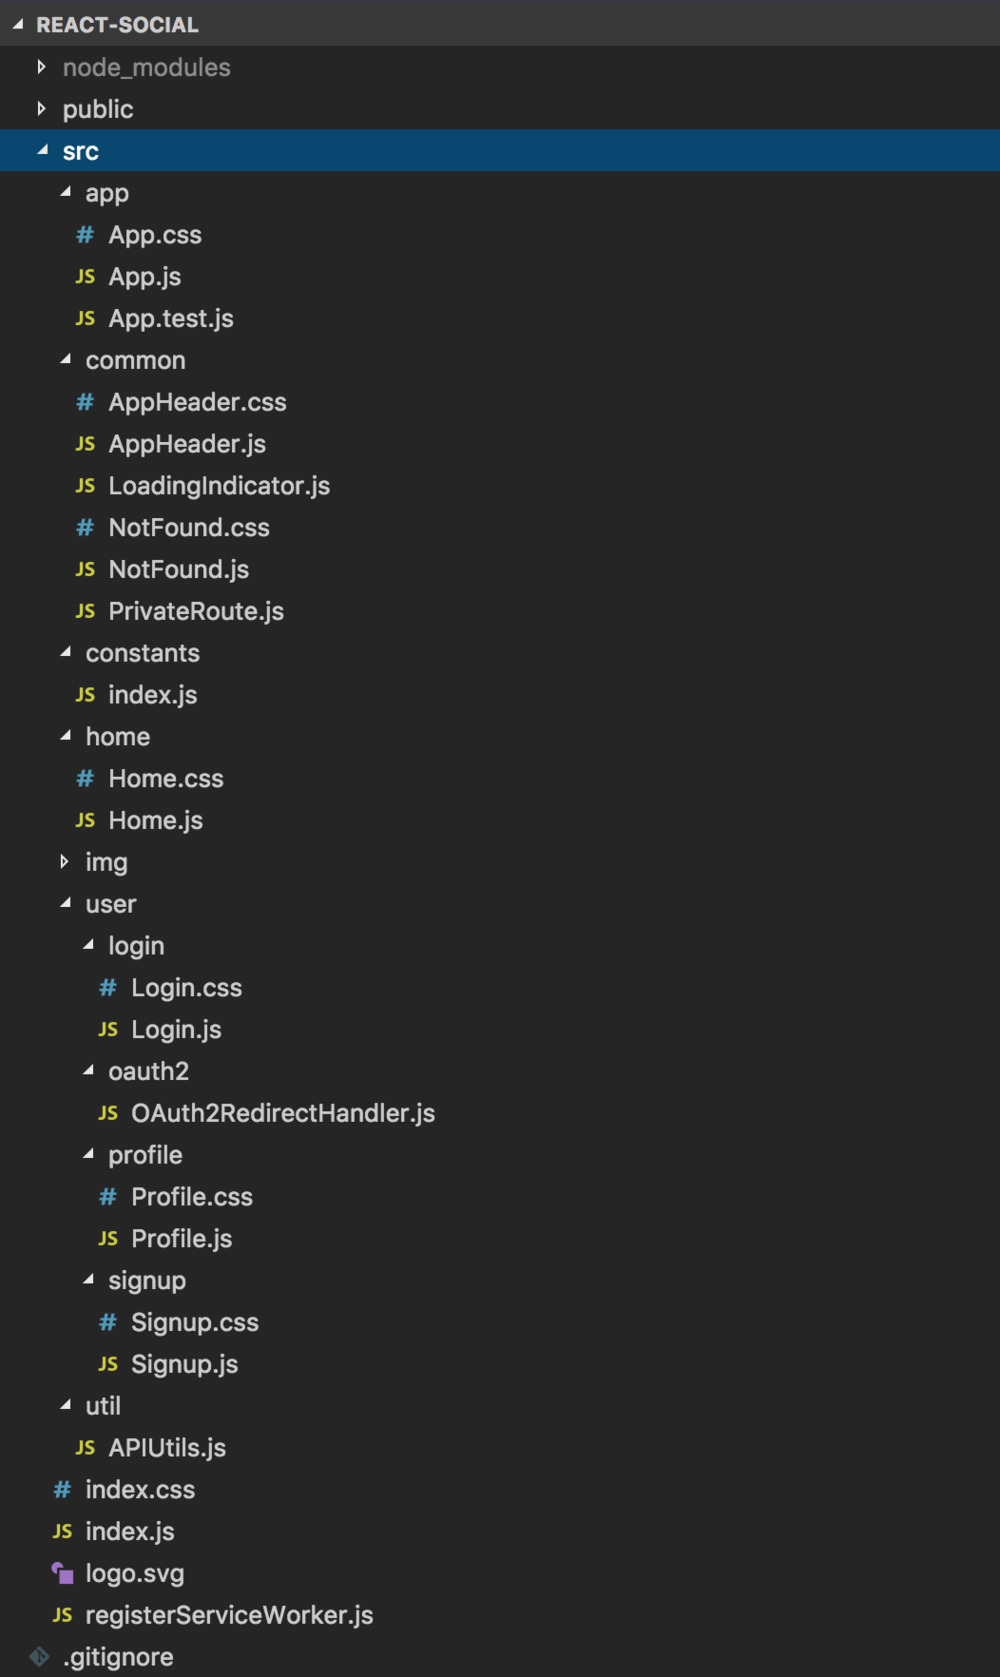
\includegraphics[width=0.31 \textwidth]{chapters/images/chp6/dirreact.jpg}
  \end{center}
  \caption{Final directory tree of the \texttt{react-social} app}
  \label{fig:dirtree}
\end{wrapfigure}

As mentioned before, this application is pretty simple and it is only used as interface between the \oauth\ Spring Boot back-end server and the user in order to display information. An alternative could be directly to implement into the Spring Boot back-end the web-server.

\noindent In order to create the base React application, simply type:
\begin{lstlisting}[language=bash]
  $ npm install -g create-react-app
  $ create-react-app react-social
\end{lstlisting}

\noindent And then add the dependencies for routing and alerts:
\begin{lstlisting}[language=bash]
  $ cd react-social
  $ npm install react-router-dom react-s-alert --save
\end{lstlisting}

\noindent That is the base React application to build on. We have to populate and organize the final directory structure in order to look like in Fig.~\ref{fig:dirtree}.

The code is pretty self-explanatory, but there are some important aspects to consider. The first one is \textbf{index.js}, that is the entry-point of the application. It renders the App component in a document object model that has \texttt{root} as id and it is subsequently wrapped into a Router to enable client-side routing. The second important aspect is \textbf{App.js}, located in \texttt{src/app}. It is the top-level element of the application and basically is responsible for the layout, the routes and manages the authentication by loading the details from the back-end of the current user, forwarding it to the child components. The \textbf{Login.js} file, located in \texttt{src/user/login}, is responsible for the \oauth\ login and the username/password login, while \textbf{OAuth2RedirectHandler.js} is the component called by the Spring Boot server when the user has completed the \oauth\ flow on it. In particular, once that the server flow is finished, the server saves all the information in a database and generates a local token. This component will receive an bearer token from the Spring Boot server (note that this token is not related to \oauth, it is a token generated by the Spring Boot server in order to manage the access to the database information) or an error otherwise.

Last but not least, the \textbf{index.js} located in \texttt{src/constants} contains the information about the endpoints. The \texttt{API\_BASE\_URL} refers to the Spring Boot server base URL, that represents the API for the \texttt{hw-client} app. The \texttt{OAUTH2\_REDIRECT\_URI} is the redirection URI where the \\ \textbf{OAuth2RedirectHandler.js} is waiting to handle the response and the three \texttt{PROVIDER\_AUTH\_URL} are the Spring Boot server URLs called when the user clicks on one of the three \oauth\ login, passing as parameter a \texttt{redirect\_uri} to let the server know where to redirect the local token once that he has completed the AuthZ Code Grant flow. 

\begin{figure}[h!]
    \centering
    \fbox{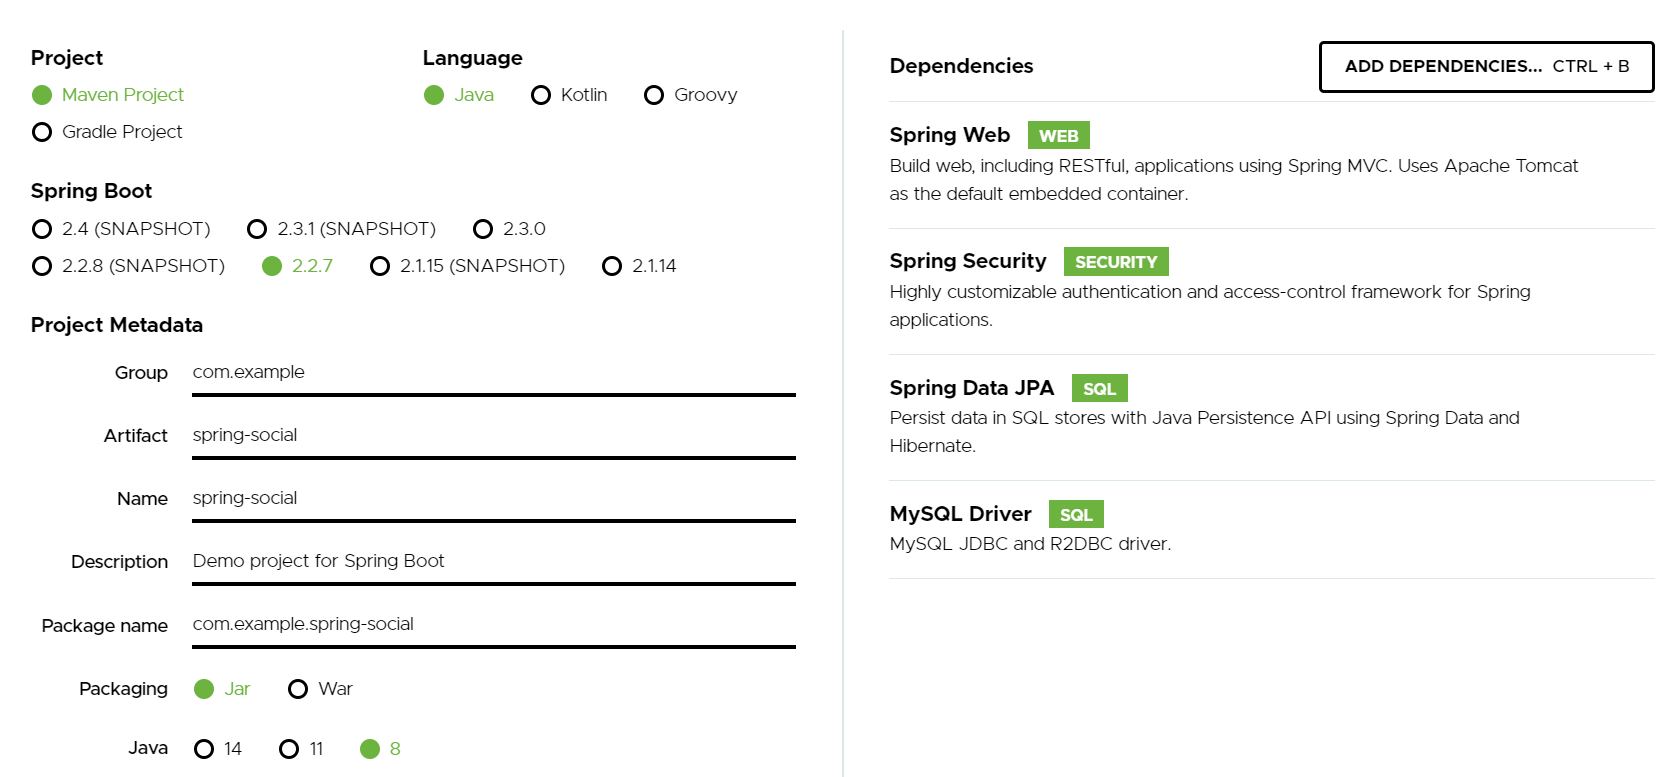
\includegraphics[width=16cm]{chapters/images/chp6/spring.png}}
    \caption{Spring Boot base project selection}
    \label{fig:spring}
\end{figure}

\subsubsection{Registration process}
In order to enable the Spring Boot server to perform a social login with an \oauth\ provider, the first step is to create an application in the provider's developer console and obtain the \texttt{client\_id} and \texttt{client\_secret}. These two strings are used by the providers (Google, Facebook and so on) to identify our server application. In addition, there are some others parameters to consider:

\begin{itemize}
    \item Authorized redirect URIs: After that the AuthZ Grant Flow is finished, the provider needs this URI in order to understand where the user has to be redirected after the flow and what are the ones that are authorized by the developer.
    \item Scopes: They represent \textbf{what} can be granted. Note that this is only meant to enable the possibility to give it, it is not automatically given to our server. The user will decide what scopes from the enabled scopes can be consumed by the Spring Boot server.
\end{itemize}

\noindent To create an app, simply start a new app in one of the following provider's page:

\begin{itemize}
    \item Google Project: \url{https://console.developers.google.com/}
    \item Facebook: \url{https://developers.facebook.com/apps}
    \item GitHub: \url{https://github.com/settings/apps}
\end{itemize}

\noindent Set the Authorized redirect URIs (more on this in the next subsection), the scopes (email, name) and retrieve the two secrets for each provider.

\subsubsection{Server-side}

\begin{wrapfigure}[15]{r}{0.3\textwidth}
  \begin{center}
    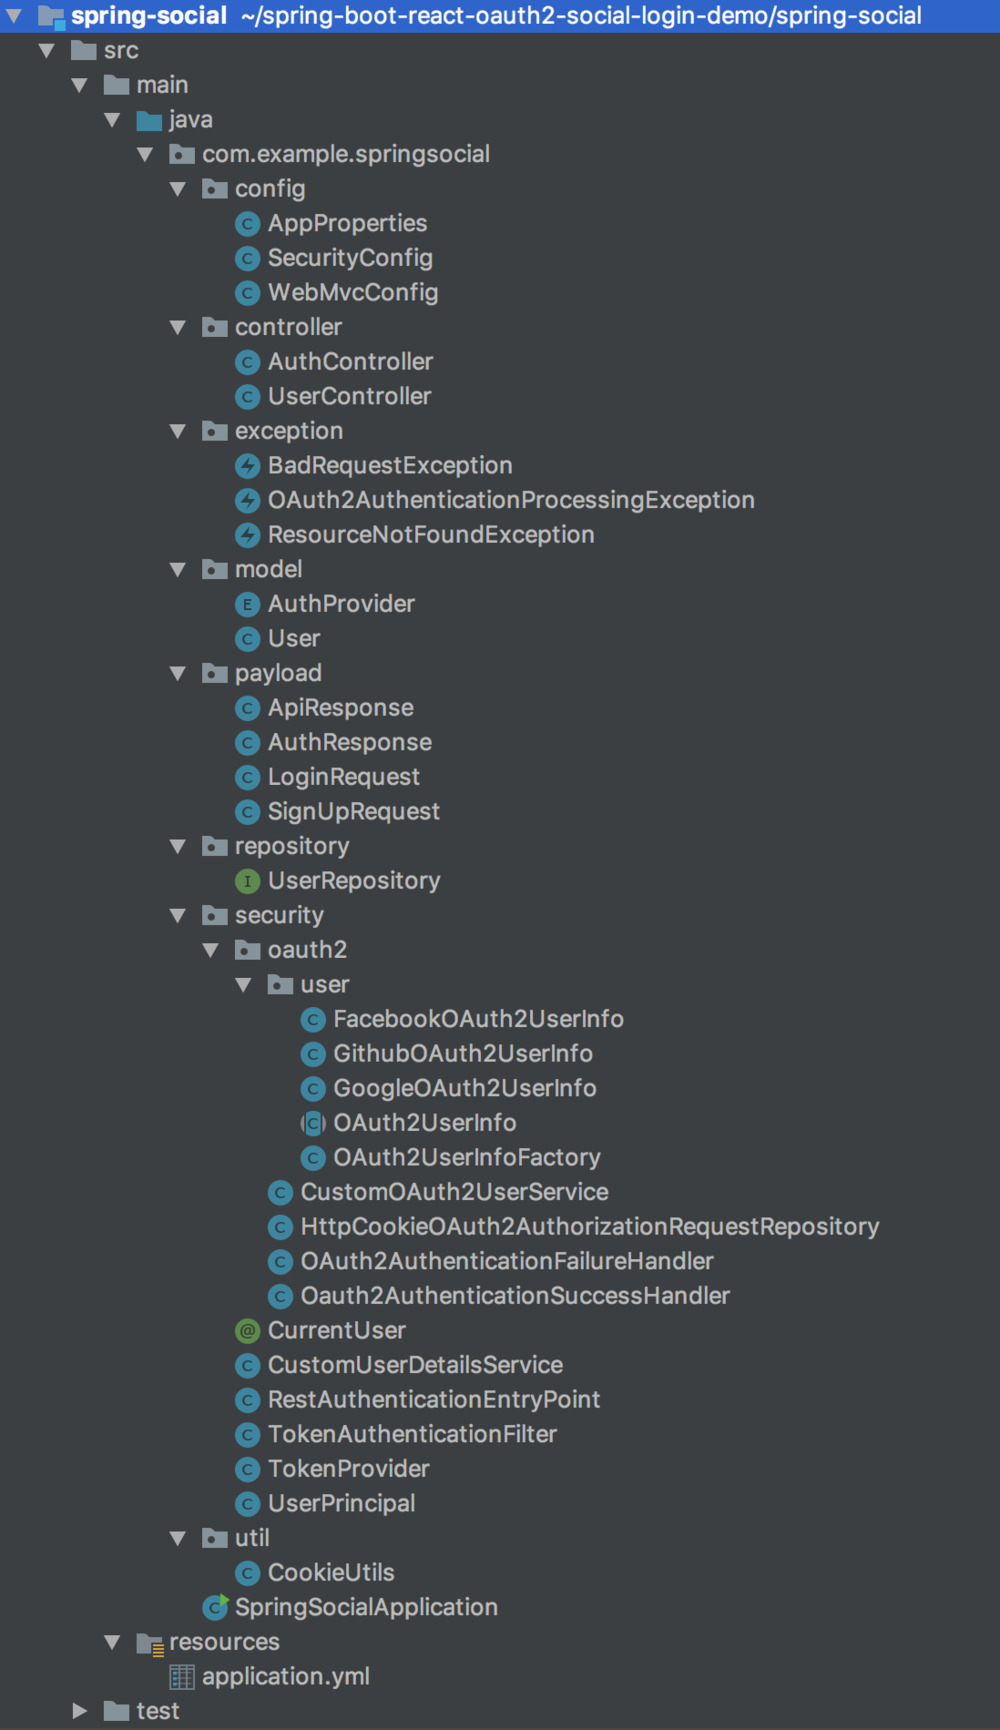
\includegraphics[width=0.3 \textwidth]{chapters/images/chp6/springdir.jpg}
  \end{center}
  \caption{Final directory tree of the \texttt{spring-social} app}
  \label{fig:dirsocial}
\end{wrapfigure}

The server, as it has already mentioned, is a Spring Boot application. The base project can be automatically created using Spring Initializr\footnote{Start the project from \url{https://start.spring.io/}}. In particular, the selection are the ones in Fig.~\ref{fig:spring}.

Then, the project folder has been modified in order to have the directory structure in Fig.~\ref{fig:dirsocial}. Furthermore, there are two more dependencies that must be added to the project (not available on Spring Initializr): \textit{\oauth\ Client} and \textit{JWT Library}. By opening the \texttt{pom.xml} file, thanks to Maven, simply add these lines into the \texttt{<dependencies></dependencies>} tags:

\begin{lstlisting}[language=XML, basicstyle=\fontsize{9}{11}\ttfamily]
  <!-- OAuth2 Client -->
  <dependency>
    <groupId>org.springframework.security</groupId>
    <artifactId>spring-security-oauth2-client</artifactId>
  </dependency>

  <!-- JWT library -->
  <dependency>
    <groupId>io.jsonwebtoken</groupId>
    <artifactId>jjwt</artifactId>
    <version>0.5.1</version>
  </dependency>
\end{lstlisting}

\noindent Now that the Spring Boot app structure is ready, we are going to analyze every Java file and configuration file in order to understand how the functionalities are implemented. The configuration file is \textbf{application.yml} (note that if a file has \texttt{.template} as extension it represents a simple file without this extension with some variables to be changed at build time, see \ref{docker} for more information). The configuration file is located in \texttt{src/main/resource/} and it contains all the information about database, redirection URIs and so on. In \texttt{spring.datasource} are saved the MySQL database variables, while in \texttt{spring.security.oauth2} we can find everything that concerns \oauth\ providers and their details. In particular, for each provider, we can insert the two secrets (\textit{clientId} and \textit{clientSecret}) with the redirect URI and the scopes.

In a few words, all the content stored in \texttt{spring:} is related to the server itself, while \texttt{app:} is used to authenticate the React web application. More in details, \texttt{app.auth} information are consumed for the creation of a JWT authentication token (that has nothing to do with \oauth) that is passed to the React front-end (or any other front-end, like a mobile app) by a redirection to \\ \texttt{http://localhost:9090/oauth2/redirect} (enabling OAuth2RedirectHandler.js) or for example \texttt{myandroidapp://oauth2/redirect} if the front-end is a mobile app.
After successfully authenticating with the \oauth\ Provider, the Spring Boot server will generate an auth token for the user and will send the token to the \texttt{redirectUri} mentioned by the front-end client in the \texttt{/oauth2/authorize} request. 

The next step is to load this configuration file and bind the properties. The \\ \texttt{@ConfigurationProperties} feature is used in \textbf{AppProperties.java} to load the \texttt{app:} information from the configuration file and is enabled with  \texttt{@EnableConfigurationProperties} in the main file \textbf{SpringSocialApplication.java}. Moreover, in order to enable CORS\footnote{Cross-Origin Resource Sharing, from "[...] a mechanism that uses additional HTTP headers to tell browsers to give a web application running at one origin, access to selected resources from a different origin.". Source: \url{https://developer.mozilla.org/en-US/docs/Web/HTTP/CORS}} is created a \textbf{WebMvcConfig.java}  so that our front-end can access the APIs from different origins. The used restrictions are pretty low for the demo, but in production environments they must be restricted.

In order to enable the database interaction, the database entities must be created. The User entity is available in the \textbf{User.java} file, alongside the \texttt{enum} \textbf{AuthProvider.java} that represents the provider. The implementation of the database functionalities is denoted to the \textbf{UserRepository.java} interface. Here it is used \textit{Spring-Data-JPA} to build a repository layer to access the database information.
Once that the configuration, the entity classes and repositories are ready, we will use Spring Security to perform the \oauth\ social login as well as the password/email based login.

The core of the \oauth\ Security on the server is \textbf{SecurityConfig.java}, that basically binds all the constituents in order to implement a security policy for the entire application. In particular, the \textit{SecurityConfig} is an extension to a  \textit{WebSecurityConfigurerAdapter} and overrides some of its methods to provide custom security configurations:

\begin{itemize}
    \item \textit{CustomUserDetailsService}
    \item \textit{CustomOAuth2UserService}
    \item \textit{OAuth2AuthenticationSuccessHandler}
    \item \textit{OAuth2AuthenticationFailureHandler}
    \item \textit{HttpCookieOAuth2AuthorizationRequestRepository}
    \item \textit{TokenAuthenticationFilter}
    \item And basically all the classes implemented in \texttt{java.com.example.springsocial.security}
\end{itemize}

\noindent The flow starts from the front-end client. After that one of the three available \oauth\ login button is clicked, the React app redirects the user to \\

\vspace{0.1cm}

\hypertarget{foo}{}

\texttt{\footnotesize{http://localhost:8080/oauth2/authorize/\{provider\}?redirect\_uri=<redirect\_uri\_after\_login>}} \\

\vspace{0.1cm}

\noindent Where \texttt{localhost:8080} is the Spring Boot server base URL, \texttt{provider} represents one of the three providers and the \texttt{redirect\_uri} is the URI to which the user will be redirected after the \oauth\ flow on the provider site (note that this redirection is not the \oauth\ \texttt{redirectionUri}).

Once that the authorization request is received, Spring Security's \oauth\ redirects the user on the \textit{AuthorizationUrl} of the \texttt{provider} with some parameters (the scopes and the redirectionUri saved in the configuration file). Here, \textit{authorizationRequestRepository} applies persistency to the request's state. The user is now on the provider's login/authorization page, where it can login and allow/deny permission to the Spring Boot server. Once that it allows it, the provider send the user to \texttt{\{baseUrl\}/oauth2/callback/provider} with an AuthZ code (or an error otherwise).

At this point, \textit{oAuth2AuthenticationFailureHandler} is invoked in case of failure (it redirects the user on the React app with an err message in the query string), otherwise the flow continues and the previous callback contains the \texttt{authorization\_code} that is automatically exchanged by Spring Security for an \texttt{access\_token}. The next step is \textit{customOAuth2UserService} that takes all the details of the authenticated user by performing HTTP GETs to the defined endpoints available in the Google/Facebook documentation and adds/updates the database. Spring Security is really useful in this objective, because it has already implemented the HTTP API calls for the most famous providers and it is almost automated. 

Finally, the last step is \textit{oAuth2AuthenticationSuccessHandler}, that creates a JWT token and sends it to the React app's \texttt{redirect\_uri} previously sent at the beginning. Once that the client app receives it, it can make a HTTP GET with the JWT on the endpoint of the Spring Boot server \texttt{/user/me} to retrieve the user information and display it to the client. The generic flow with Google is available in \texttt{.svg} format\footnote{\url{https://github.com/nopesir/oauth-hw-security/releases/download/v0.5-alpha/flow.svg}}.


In the Section \ref{csrf} has been discussed the problem of CSRF. In particular, the recommended way of avoiding this kind of attack is the use of a \texttt{state} parameter. When the Spring Boot server redirects the user to the provider's login page (see \hyperlink{foo}{here} the HTTP redirection link), it has to first generate this string variable and send it as HTTP parameter with the \texttt{redirect\_uri}. The provider must return this parameter unaltered in the \oauth\ callback and the server will compare the generated one with the received one. In case they don't match, the flow is stopped and the request denied.
The class \textit{HttpCookieOAuth2AuthorizationRequestRepository} temporary stores the \texttt{redirection\_uri} and the \texttt{state} params in a short lived cookie.

To gain access to the user's personal info, the \textit{CustomOAuth2UserService} implements the Spring Security's \textit{DefaultOAuth2UserService} by its \texttt{loadUser()} method (called after that a \oauth\ \texttt{access\_ token} is finally available). More in details, the method fetches what is needed from the provider and then checks the database in order to update it. Since the JSON structure of the responses of each provider changes, Spring Security provides a parsing layer that returns a map of key-value pairs. In order to manage the different providers, a generic \textit{OAuth2UserInfo} is created and a factory design pattern is implemented through \textit{OAuth2UserInfoFactory} in order to instantiate the correct \textit{OAuth2UserInfo} (\textit{GoogleOAuth2UserInfo}, \textit{FacebookOAuth2UserInfo}, \textit{GithubOAuth2UserInfo}).

In addition to the \oauth\ login, the Spring Boot server implements the classic email/password based authentication. The class \textit{AuthController} is responsible for controlling the REST endpoints \texttt{/auth} and \texttt{/signup}, while the \textit{CustomUserDetailsService} implements \textit{UserDetailsService} in order to load the user from the database. In order to manages (generate/verify) the JWT tokens, a \textit{TokenProvider} is created. Moreover, the \textit{TokenAuthenticationFilter} class uses the provider one to verify the JWT and set the \texttt{SecurityContex}. \textit{RestAuthenticationEntryPoint} checks for unauthorized accesses and returns a 401 HTTP error for it. The \textit{UserPrincipal} class contains the details of the authenticated user while \textit{UserController} implements the API for retrieving the details of it. Finally, there is a utility class that is used for the cookies management called \textit{CookieUtils}. \textit{LoginRequest}, \textit{SignUpRequest}, \textit{AuthResponse} and \textit{ApiResponse} are the request/response payloads.

For further information on Spring Security, see the documentation \cite{sprsec}.
% ------ END OF SECTION B.2.1 ------

% ------ SECTION B.2.2 ------
\subsection{\oauth\ with custom AuthZ/Resource servers}
This second implementation example is required in order to better understand \oauth\ and his actors without the customization of providers like Google. It is possible to build an authorization server and a resource server using the \textit{authorization grant flow} (\ref{authcg}). For this task, before using direclty the \rfc{6749}, the developer.okta.com's article "What is the OAuth 2.0 Authorization Code Grant Type?" \cite{oauth2} is a good start. The demo is composed by three servers:

\begin{itemize}
    \item \textit{Client-server}, that acts like the Spring Boot server in the previous example (the client of the \oauth\ protocol specification that is interested in accessing a resource), but without a React web app: it is used a classic routing website served directly from the server itself.
    \item \textit{Authorization-server}, that provides endpoints for user authentication and authorization, token access and token refresh and so on.
    \item \textit{Resource-server}, that makes available resources by using the retrieved token from the authorization server.
\end{itemize}

Clearly, there is the user too (the resource owner), that is responsible for grant/deny permissions to the client-server. All the software of this demo uses Maven for project management, dependencies and so on. Moreover, it is built on top of \texttt{Jakarta EE} \cite{jaksec} with \texttt{MicroProfile}, but more details are available in the dedicated subsections. 

\subsubsection{Client-server}
This web-server implements four Servlets\footnote{Exploit dynamic web content with Java, "[..] class that is used to extend the capabilities of servers that host applications accessed by means of a request-response programming model.". Source: \url{https://docs.oracle.com/javaee/5/tutorial/doc/bnafe.html}}:

\begin{itemize}
    \item Request the authorization code from the authorization server's endpoint.
    \item Request the access token by consuming the authorization code.
    \item Request the access token by consuming the refresh token (\ref{accref}).
    \item Request the resource from the resource server's endpoint by consuming the access token.
\end{itemize}

\noindent Moreover, it uses MicroProfile Config for configuration files injection and JAX RS Client for accessing web resources. For simplicity, the \texttt{client\_id} and \texttt{client\_secret} are manually defined in the authorization server as it will be explained in the next subsection. This means that our client must have securely stored the two secrets that, for this demo, are only one pair (since the client is only one). In the configuration file stored in \texttt{META-INF/microprofile-config.properties} (it must be noted that it applies the same \texttt{.template} design, as explained in the first demo), apart from the secrets, other important variables are:

\begin{itemize}
    \item \texttt{redirect\_uri}: As it was already mentioned, this is \textit{where} to receive the AuthZ code.
    \item \texttt{scope}: The permission requested by the client.
    \item \texttt{authorization\_uri}: The client needs to know where to send the request for the AuthZ code.
    \item \texttt{token\_uri}: As for the AuthZ URI, the client needs to know where to send the request to exchange the code for an access token.
\end{itemize}

\noindent It is important though to point out that the URIs are configured for the Docker virtualized network and for a normal run without Docker they must be changed.

The first Servlet implements the AuthZ code request on the AuthZ server's endpoint and it is represented by the \textit{AuthorizationCodeServlet} waiting to start on the \texttt{/authorization} endpoint of the client. More in details, the Servlet creates and stores the \texttt{state} param, retrieves the information from the MicroProfile Config file and builds the URI attaching all the variables. Finally, it redirects the user to the built URI (that is on the AuthZ server). After processing the request, the AuthZ server will redirect back the user to the client with the AuthZ code and the same \texttt{state} param on the URI \texttt{http://localhost:9180/callback?code=tughdj57gh5hfd\&state=57t7fdhgwejgu54h} where the second Servlet is waiting for the AuthZ code (the client server is on 9180, the AuthZ server is on 9080 and the resource server on 9280).

The second Servlet starts as soon as the AuthZ server redirects back to \texttt{/callback} with the AuthZ code and the \texttt{state} as parameters. The implementation is in class \textit{CallbackServlet}. First, it checks the \texttt{state} match and then it uses the received code to request an access token. In this case there is no browser interaction, it is all implemented through HTTP POST and JAX RS Client: here the token endpoint requires the two secrets too in the \textit{Authentication} header, along with the code, the type of the code and the redirect URI. Now the client has the access token (and the refresh token too) and it can access information on the resource server by using the third Servlet implemented in \textit{DownstreamCallServlet} waiting on \texttt{/downstram} with two actions passed as query params: \textit{read} or \textit{write}. Based on the action, the Servlet calls the resource server's APIs with the access token in the Authorization HTTP header and receives a string if it has access or an HTTP Forbidden error if it does not.

The last Servlet is used to obtain a new access token starting from the refresh token. This is really useful because it does not requires the user to repeat all the flow, it does not require the user at all! The Servlet is ready to start at \texttt{/refreshtoken} and, similarly to the code of \textit{CallbackServlet}, it uses only JAX RS Client and HTTP POST to build the request, that has the refresh token, the scopes and as grant type \texttt{refresh\_token}. It is necessary the Authentication header with the secrets too. The request is posted on the same token endpoint of the AuthZ server, but the AuthZ server will know what to do because of the \texttt{grant\_type} param. If the response is 200 HTTP, the new token is stored and it can be used for the next calls to the resource server.

In order to start the first Servlet and/or to know every parameters and tokens for educational purposes, a simple homepage is built (\texttt{src/main/webapp/index.jsp}) that in a few words prints all the information and makes available the endpoints (by mouse click) to the user.

\subsubsection{Authorization-server}
This server is the core of the \oauth\ implementation. For simplicity a pre-configured client and a pre-configured user are used, stored in \texttt{src/main/resources/data.sql.template} (it must be pointed out though that for a production environment the passwords must be hashed). 

The first important endpoint is the AuthZ endpoint that is responsible for the authentication of the user in order to subsequently ask for the needed permissions. The Section 3.1 of the \rfc{6749} states that "The authorization server MUST support the use of the HTTP "GET" method [\rfc{2616}] for the authorization endpoint and MAY support the use of the "POST" method as well.". In this implementation is preferred the HTTP GET method alone. Since the specification does not asks for a particular login flow, a simple login form with Jakarta EE Security can be used. The class \textit{AuthorizationEndpoint} contains:

\begin{itemize}
    \item \texttt{@FormAuthenticationMechanismDefinition} in order to ensure that the user is logged to proceed.
    \item HTTP GET Servlet that checks the validity of the secrets, the redirect URI, the requested scope and saves all this params in the session and redirects the user to the \texttt{authorization.jsp} from where it selects what to authorize with some checkboxes.
    \item HTTP POST Servlet that receives the user checkboxes from \texttt{authorization.jsp}, uses the saved params in the preceding point to populate a new AuthZ code model with the authorization code, the \texttt{client\_id}, the approved scopes, the expriration date and so on and redirects back to the client on the \texttt{redirect\_uri} by adding to the query params the new code alongside the state received at the beginning for avoiding CSRF. The \texttt{redirect\_uri} must exist in the table as an authorized URI for redirections.
\end{itemize}

\noindent As mentioned before, to retrieve the access token starting from the authorization token is an action that does not require the user nor the browser intervention. The token endpoint of the AuthZ server, in accordance with the client server, uses JAX RS to expose the endpoint. The class \textit{TokenEndpoint} implements the next step of the workflow: retrieve the access token. The Servlet accepts only HTTP POST and, as mentioned in the \oauth\ specification, accepted parameters mus be \texttt{application/x-www-form-urlencoded}. The first thing that the Servlet checks is the \texttt{grant\_type} that must be \texttt{authorization\_code} since this is an AUthZ Code Grant flow implementation. The second check is on \texttt{client\_id} and \texttt{client\_secret} that are in the Authorization header of the received post (this is required by the protocol in order to identify the client). The two secrets are ecoded into Base64url following this conversion:
\begin{lstlisting}
  BASE64URL(client_id:client_secret)
\end{lstlisting}

\noindent Finally the Servlet creates the access token by using \textit{AuthorizationCodeGrantTypeHandler}. 

Since the endpoint can and should be used for both the requests of getting an access token starting from an authorization code or getting an access token starting from a refresh token, the Servlet must be dynamically capable of chosing the right class instance. A possible solution is the implementation through the Contexts and Dependency Injection (CDI). More in details, an \textit{AuthorizationGrantTypeHandler} interface is created and implemented with \textit{AuthorizationCodeGrantTypeHandler} for AuthZ code to access token and with \textit{RefreshTokenGrantTypeHandler} for refresh token to access token. Each class is decorated with the \texttt{@Named} that specifies for the first one the \texttt{authorization\_code} type and for the second one the \texttt{refresh\_token} type. By using the decoration, in the Servlet can be written a single line of code that uses the received string (\texttt{grantType}) on the endpoint and uses it directly to load one handler or the other one:

\noindent \texttt{\footnotesize{AuthorizationGrantTypeHandler authorizationGrantTypeHandler= \\
\indent authorizationGrantTypeHandlers.select(NamedLiteral.of(grantType)).get();}} 

\noindent In order to generate tokens though, it is required that the server signs them with a private RSA key. It has been used OpenSSL to generate the private key:

\begin{lstlisting}[language=bash, basicstyle=\fontsize{9}{11}\ttfamily]  
  $ openssl genpkey -algorithm RSA -out private-key.pem -pkeyopt rsa_keygen_bits:2048
\end{lstlisting}

\noindent And the path to this key is saved in \texttt{resources/META-INF/microprofile-config.properties} in order to be injected into the server configuration info in order to be loaded directly from the code. Alongside the private key, a corresponding public key is generated:

\begin{lstlisting}[language=bash, basicstyle=\fontsize{9}{11}\ttfamily]  
  $ openssl rsa -pubout -in private-key.pem -out public-key.pem
\end{lstlisting}

\noindent And stored in the same configuration file.

When the resource server receives a request with an access token for a resource, it has to verify it by using the public key. Another endpoint is necessary on the AuthZ server: a JWK [\rfc{7517}] for public key distribution. This endpoint is mapped in \texttt{/jwk} and the Servlet is implemented by the class \textit{JWKEndpoint}. Thanks to the Nimbus library, the code is much more simplified with both the JWT and PEM formats compatibility (by specifying the param \texttt{format} in the URI query).

For what concerns the authorization endpoint, it was already mentioned the existence of the \texttt{AuthorizationGrantTypeHandler}, but how does it work? What does the endpoint returns? More in details, it uses the Nimbus JOSE library for creating a JWT token. The first thing to do is to create a JWT header and then populate the payload with some claims (like the issuer, the claimer and so on). Then, the token must be signed with the RSA Private Key. This step can be divided in two: 

\begin{itemize}
    \item The JWT is created starting from the claims and the header.
    \item The \textit{RSASSASigner} object uses the imported PEM key to sign the JWT.
\end{itemize}

\noindent Finally, the JWT is ready and it is serialized into a \textit{String}. More in details, this serialization follows the "JWS Compact Serialization" defined in Section 7.1 of the \rfc{7515} \cite{RFC7515}:

\begin{lstlisting}
  BASE64URL(UTF8(JWS Protected Header)) || '.' ||
  BASE64URL(JWS Payload) || '.' ||
  BASE64URL(JWS Signature)
\end{lstlisting}

\noindent An example of a valid serialized JWT for this implementation could be:

\begin{lstlisting}
  eyJ0eXAiOiJKV1QiLCJhbGciOiJSUzI1NiJ9
  .
  eyJzdWIiOiJhcHB1c2VyIiwiYXVkIjoiaHR0cDpcL1wvMTcyLjI4LjEuMzo5Mjg
  wIiwidXBuIjoiYXBwdXNlciIsIm5iZiI6MTU5Mzc5MDY1MSwic2NvcGUiOiJyZX
  NvdXJjZS5yZWFkIiwiaXNzIjoiaHR0cDpcL1wvMTcyLjI4LjEuMjo5MDgwIiwiZ
  3JvdXBzIjpbInJlc291cmNlLnJlYWQiXSwiZXhwIjoxNTkzNzkyNDUxLCJpYXQi
  OjE1OTM3OTA2NTEsImNsaWVudF9pZCI6IndlYmFwcGNsaWVudCIsImp0aSI6ImI
  3MmNiOTc2LTgxY2ItNGRjNi1hMjMwLTg2YzE2ZTE1NWQyNiJ9
  .
  pVjwobEPgfjLMdVHdBKNhwNcqpG9UytZH2wcJYtVuVFitgaDk6cWwTCCJlOLLO
  qcvtXsl4RjXavKFFGVIalQL1Smqj69u6i98VqRVn6yRiPyi8EDJeJn6Xa2BjIF
  ePjPc8EyejvM47F0LDwJO19kb-s8fcXKqEdB0zTQ8vMvb-1jgk9KlXWzsT3HxN
  rRLnpHyUAWjELVe30awwF0v9MfGPdxX64Kq62hNA2hg8TLLHXWEgU1v5eqCmdk
  sD1kyhS_cPSQLRKcXQMDPdTe1H4cnXnm8Gl_qYV885RYLx0DXqddWoiRPCLu
  5RbLr2ZXxAOSFQ8kKScmXX3BUpkiHS5afw

  
\end{lstlisting}

\noindent Where the first part of the string is the Base64url encoded JOSE Header that specifies the used algorithm and the type. The decoded string would be:

\begin{lstlisting}
  {
    "typ":"JWT",
    "alg":"RS256"
  }
\end{lstlisting}

\noindent The second part represents the encoded JWS Payload with all the previously built claims, decoded as:

\begin{lstlisting}
  {
    "sub":"appuser",
    "aud":"http://172.28.1.3:9280",
    "upn":"appuser",
    "nbf":1593790651,
    "scope":"resource.read",
    "iss":"http://172.28.1.2:9080",
    "groups":["resource.read"],
    "exp":1593792451,
    "iat":1593790651,
    "client_id":"webappclient",
    "jti":"b72cb976-81cb-4dc6-a230-86c16e155d26"
  }
\end{lstlisting}

\noindent Where, according to the \rfc{7519}\ specification \cite{RFC7519}, are defined the following Registered Claim Names:

\begin{itemize}
    \item \texttt{sub}: OPTIONAL. The principal that is the subject to the JWT.
    \item \texttt{aud}: OPTIONAL. Audience, to whom the JWT is addressed.
    \item \texttt{nbf}: OPTIONAL. Not Before, "the time before which the JWT MUST NOT be accepted for processing." \cite{RFC7519}
    \item \texttt{iss}: OPTIONAL. The issuer of the JWT.
    \item \texttt{exp}: OPTIONAL. The expiration time.
    \item \texttt{iat}: OPTIONAL. Issued At.
    \item \texttt{jti}: OPTIONAL. JWT ID, unique identifier for the JWT.
\end{itemize}

\noindent And the following Private Claim Names designed for the demo:

\begin{itemize}
    \item \texttt{upn}: To be mapped into Jakarta EE Security \textit{CallerPrincipal}.
    \item \texttt{groups}: To be mapped into Jakarta EE \textit{Roles}.
    \item \texttt{client\_id}: The ID of the \oauth\ web-server client.
\end{itemize}

\noindent These claims are built in the token endpoint response code in the \textit{AbstractGrantTypeHandler} class. For what concerns the \texttt{refresh\_token}, the JWT is similar, with few claims and an expiration of one day.
Finally, the third and last part of the JWT represents the Base64url encoded JWS Signature performed by the server on the following octets:
\begin{lstlisting}
  ASCII(
    BASE64URL(UTF8(JWS Protected Header)) || '.' ||
    BASE64URL(JWS Payload)
  )
\end{lstlisting}

\noindent Those octets are signed using RSASSA-PKCS1-v1\_5 with the SHA-256 hash algorithm (defined as \texttt{RS256} in the JOSE Header) by the server and finally encoded in Base64url.

The last thing to do is build the JSON response and add the elements and the serialized JWTs (refresh and access tokens) in order to return the information requested by the client. This step is implemented into the \textit{AuthorizationCodeGrantTypeHandler} class, that once it has serialized the two JWTs, it builds the response:

\begin{lstlisting}[language=bash, basicstyle=\fontsize{12}{14}\ttfamily]
  {
    "access_token": "averylongstring,seepage46" ,
    "token_type": "Bearer",  
    "expires_in": 1800,
    "scope": "resource.read",
    "refresh_token": "smallerthanaccesstoken,lessclaims"
  }
\end{lstlisting}

A detailed diagram of the AuthZ Code Grant flow for this implementation is available in the resources as \texttt{flow\_access-token.svg}\footnote{\url{https://github.com/nopesir/oauth-hw-security-custom/releases/download/v1.0/flow_access-token.svg}}, while a detailed diagram of the Refresh Token flow is available in the resources as \texttt{flow\_refresh-token.svg}\footnote{\url{https://github.com/nopesir/oauth-hw-security-custom/releases/download/v1.0/flow_refresh-token.svg}}.

\subsubsection{Resource-server}
This third and last server exposes the APIs to the client for accessing the user's information by consuming the access token retrieved in the previous steps. This server uses JAX RS and MicroProfile. In particular MicroProfile JWT is responsible for the validation and the mapping of the scopes in Jakarta roles. Thanks to these libraries, the code is pretty simple. In particular, the class \textit{OAuth2ResourceServerApplication} is decorated with \texttt{@DeclareRoles} to define the scopes available and \texttt{@LoginConfig} to specify the authentication method. Finally, the class \textit{ProtectedResource} represents the resource (in terms of called function) that can be personalized in order to return a file or any other protected information (in this example, it is a string).

It must be pointed out that even if the AuthZ server implements the JWT endpoint, it has been chosen to add the key directly in the server's resources (in order to use the endpoint, the path in the configuration file has to be replaced with the endpoint of the AuthZ server).
% ------ END OF SECTION B.2.2 ------
% ------ END OF SECTION B.2 ------

% ------ SECTION B.3 ------
\section{Dockerization}
To best manage, debug and deploy the two solutions, it has been chosen to dockerize the single servers. More in details, every module has its own \texttt{Dockerfile} and each demo has its \textit{docker-compose-build.yaml} to build and run at the same time all the modules with the network configuration. Moreover, the pre-built images are available on Docker Hub and a special \texttt{docker-compose.yaml} for each solution can be used to rapidly pull all the images without wasting time to build (this is mainly done for the User Guide to rapidly test and run the examples).

% ------ SECTION B.3.1 ------
\subsection{\oauth\ with Google/Facebook}
The first demo has two modules: the React web-app and the Spring Boot JAVA server. Each of them has its \texttt{Dockerfile}. In particular, in the React web-app, there is a two-staged docker build:

\begin{itemize}
    \item The app is built by using as base image \texttt{node:12.4.0-alpine}, producing the web-app.
    \item The web-app is copied in a simple \texttt{nginx:1.17.0-alpine} image that implements the NGINX server alongside a standard \texttt{nginx.conf}, exposing the tcp/9090 port to \texttt{localhost}.
\end{itemize}

\noindent In the Spring Boot server, the approach is similar:

\begin{itemize}
    \item The server is built using as base image \texttt{openjdk:8-jdk-alpine} with the \texttt{mvnw} command (Maven Wrapper). Moreover, the configuration files are modified according to the different arguments passed.
    \item After that the application is packed in a \texttt{.jar}, the second stage uses \texttt{openjdk:8-jre-alpine} (a minimal image) to copy the package and run the server once that the container starts up.
\end{itemize}

These \texttt{Dockerfile}s are not meant to be used singularly but through \texttt{docker-compose}. The \texttt{docker-compose-build.yaml} file is responsible to use each \texttt{Dockerfile} to build the images, expose the containers in predefined ports and create some basic container network configuration. To start the local build and run the demo, the command is

\begin{lstlisting}[language=bash, basicstyle=\fontsize{12}{14}\ttfamily]
  $ docker-compose -f docker-compose-build.yaml up
\end{lstlisting}

\noindent That builds everything from scratch. The command needs time (there are some tasks like \texttt{npm install} that are heavy), but in the end, the two modules will be ready to test. The \texttt{docker-compose.yaml} can be used instead for a 
quicker run without build.

It is really important to type the same command with the \texttt{down} option when the test is finished in order to release all the residual resources of Docker.
% ------ END OF SECTION B.3.1 ------

% ------ SECTION B.3.2 ------
\subsection{\oauth\ with custom AuthZ/Resource servers}
The dockerization design of the second example is identical to the first one: a \texttt{Dockerfile} for each server module that are used only by the \texttt{docker-compose-build.yaml} to entirely build and run locally the solution. The three servers use Open Liberty as server runtime, integrated with the project as Maven dependency. Moreover, some arguments are editable from the compose to correctly print personalized version of the configuration file (e.g. for the user definition or for the secrets definition).

The network namespace is configured as a simple LAN on \texttt{172.28.0.0/16} and the three servers are placed as follows:

\begin{itemize}
    \item Client server: 172.28.1.1 on tcp/9180
    \item AuthZ server: 172.28.1.2 on tcp/9080
    \item Resource server: 172.28.1.3 on tcp/9280
\end{itemize}

The client and the authorization servers have the exposed ports on the local guest machine to be reachable from the user during the redirections of the protocol itself. The resource server is not accessible from the host, but only indirectly from the client server through its APIs and using the access tokens (to provide basic isolation of the resources).
\label{docker}

Finally, to analyze and debug the messages exchanged in the Docker LAN, it has been used the \texttt{netshoot} \cite{netsh} container tool alongside \texttt{termshark} \cite{terms}. To catch all the HTTP exchanged messages from one of the three containers, simply run:
\begin{lstlisting}[basicstyle=\ttfamily]
  $ docker run -it --rm --net \ 
  $ container:<container_name> \ 
  $ --cap-add=NET_ADMIN --cap-add=CAP_NET_RAW nicolaka/netshoot \
  $ termshark -i eth0 -Y http
\end{lstlisting}

% ------ END OF SECTION B.3.2 ------
% ------ END OF SECTION B.3 ------

% ------ END OF APPENDIX B ------